\documentclass[onecolumn, groupedaddress, 10pt]{revtex4-1}
\usepackage[utf8]{inputenc}
\usepackage{amsmath}
%\usepackage{mathtools}											% For putting boxes around equations "\Aboxed{}"
\usepackage{amsfonts}
\usepackage{amssymb}
\usepackage{graphicx}											% Use pdf, png, jpg, or eps§ with pdflatex; use eps in DVI
\usepackage[left=2cm, right=2cm, top=2cm, bottom=2cm]{geometry}
\usepackage{float}												% for controlling the position of objects ie. tables

%\usepackage{breqn}

%\usepackage{color}												% For adding color to equations ex.: "/color{red}"

\usepackage[small, bf]{caption}									%Adjust caption size of figures, tables, pictures...
\setlength{\captionmargin}{15pt}
										
\graphicspath{{images/}{earthMotionModulationFigure/}}			% folder where images are stored in current directory


% --------------------------- Code for placing two figure side by side ------------------------------------------------------------------
\usepackage{caption}
\usepackage{subcaption}

% --------------------------- Code for the bibliography ---------------------------------------------------------------------------------
\usepackage{natbib}												% For fancy in-text citations
\bibliographystyle{plain}



\begin{document}

\author{Curtis Rau}
\author{Colin Gordon}
\author{David Witalka}
\author{Samuel Akwei-Sekyere}
\affiliation{Michigan State University}
\title{A Novel Method for Removing the Cyclic Frequency Shift due to the Earth's Motion about the Sun from Astronomical Continuous-Wave Data}

\begin{abstract}
This senior thesis is presented to Michigan State University for partial fulfillment of the requirements for a baccalaureate degrees in Physics and Neuroscience.
In this paper we will introduce the Gustafson Algorithm for removing frequency/phase modulation form a signal.  This method is powerful because it works in the frequency rather than time domain (explain why this is an advantage).  Here we will focus on its applications to LIGO, but there are many applications.  Some other examples are:
-Radio wave astronomy
-Comunications systems using FM?
-What are some other possible applications??

-we are given time series data.
-we are looking for phase modulated gravitational waves.
-form of phase modulation depends on the nature of the binary orbit.
\citep{Saulson}
\citep{LSCall}
\citep{Deanna}
\citep{folland}
\citep{griffiths}
\end{abstract}

\maketitle

% --------------------------- Code for the Cover Page ---------------------------------------------------------------------------------

\pagebreak

\section*{Division of Labor}

\textbf{Curtis Rau}
\begin{itemize}
\item organized topics and problems of interest, directed group research
\item wrote algorithm and discussion of results
\item made figures for presentation and paper
\item wrote rough draft and template for paper
\item Wrote the C++ implementation
\end{itemize}


\textbf{Colin Gordon}
\begin{itemize}
\item researched and solved phase modulation of astronomical signal caused by rotation of earth using circular orbit approximation
\item wrote introduction
\item reviewed paper and edited
\end{itemize}

\textbf{David Witalka}
\begin{itemize}
\item created and organized presentation slides
\item researched and edited sections on sampling theorem, Nyquist Frequency and aliasing, Carson’s rule
\item reviewed paper and edited
\end{itemize}

\textbf{Samuel Akwei-Sekyere}
\begin{itemize}
\item reviewed and expanded paper
\item researched and wrote sections on error and noise analysis
\end{itemize}

\pagebreak


\section{Introduction}
Einstein published his theory of general relativity in 1915. A consequence of his theory was that space time could stretch and contract when acted upon by a gravitational source. It didn't take long then to realize that under the right conditions this stretching and contracting could cause waves through the very fabric of spacetime. Go forward nearly 100 years and the very first evidence for these waves existing is discovered by the LIGO detector. They measured the ripples in space due to two massive black holes inspiralling and finally colliding together in an event that consumed 30 solar masses. This confirmed Einstein's theory and now the field of gravitational astronomy has been born. It is believed that gravitional wave sources are actually fairly common in our universe and sources of continuous monochromatic (one frequency) gravitational radation are predicted to exist; at least sources whose frequency wonders over many periods \cite{}. If they do exist they are apparently very low intensity as viewed from earth because none have been observed to date \cite{}. There is one phenomena in particular that may be significantly repressing the amplitude of these signals as seen from Earth. This would be frequency modulation.  When a wave is frequency modulated, its power is distrbuted amongst an infinite number of sidebands which are the frequencies measured when taking Fourier Transform of the data that comes from the sinusoidal phase shift due to the Doppler effect from Earth's motion relative to the source. To calculate frequency observed for a gravitationl wave we need to think about the source as an object that is Megaparsecs away (potentially in other galaxies). they are so far that their Sphereical coordinate will not change significantly and the object will move relative to the sun with nearly constant velocity over the time we collect data. This means that the sun will see the monochromatic wave produced by the source as monochromatic. Based on this and that the waves travel at the speed of light can write the wave as a lorentz invariant 4 vector.


%-- INTRODUCTION TO LIGO AND GRAVITATIONAL RADATION HERE --

%Sources of continuous monochromatic (one frequency) gravitational radation are predicted to exist; at least sources whose frequency wonders over many periods \cite{}.  If they do exist they are apparently very low intensity as viewed from earth because none have been observed to date \cite{}.  One phenomena may be (significantly??) repressing the amplitude of these signals as seen from Earth.  This would be frequency modulation.  When a wave is frequency modulated, its power is distrbuted amongst an infinite number of sidebands which are the frequencies measured when taking Fourier Transform of the data that comes from the sinusoidal phase shift due to the Doppler effect from Earth's motion relative to the source.  There are two reasons to believe frequency modulation is truly occuring (reword).  

%Recently the discovery of gravitational waves was announced.  We have reason to believe the most numerous sources of gravitational waves in the universe are compact stars (like Black holes and Neutron Stars).  These stars are expected to emmit single frequency waves over very long periods of time.  It is also believed that roughly half of all neutron stars are in binary systems, ie. two of them orbiting around eachother.  This phase modulates the signal which has the effect of reducing the power in the carrier frequency and distributes it into higher and lower harmonics.  This spreads out the power of the signal over a range of frequencies which makes it harder to detect these waves.  Especially because there is a high noise to signal ratio in the LIGO data.

%To calculate frequency observed for our wave we need to think about the source as an object that is Megaparsecs away (potentially in other galaxies). they are so far that their Sphereical coordinate will not change significantly and the object will move relative to the sun with nearly constant velocity over the time we collect data. This means that the sun will see the monochromatic wave produced by the source as monochromatic. Based on this and that the waves travel at the speed of light can write the wave as a lorentz invariant 4 vector.   

\begin{figure*}[b]
	\centering
	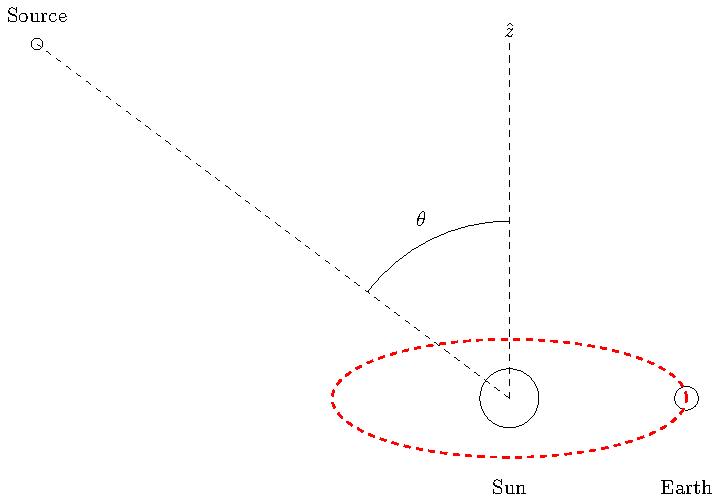
\includegraphics[width=.75\linewidth]{earthMotionModulationFigure.pdf}
	\caption{\label{fig:earthMotionModulationFigure}}
\end{figure*}

%-The equivalence of the two ways of looking at it.
%-The boost is in the arbitrarily chosen x direction, and the velocity is with respect to the sun's frame of rest.

We introduce some variables: $\Gamma$ is the modulation index, $\omega_e$ is the angular frequency of the Earth's rotation about the Sun, $\omega_0$ is the frequency of the wave to be detected, $\phi_0$ is the phase of the wave to be detected at $t=0$, $\phi_e$ is the relative phase difference between the Earth's rotation about the Sun and the wave to be detected. in the equation below we use theta as the polar angle from the axis perpendicular to the orbit of Earth, gamma is the lorentz factor from special relativity. beta is the velocity of Earth's orbit divided by the speed of light. $\mathbf{K}$ is the four vector of the wave's frequency and wave number.

\begin{align}
\label{eqn: new k}
\mathbf{K} &=
\left( \begin{array}{cccc}
	    \gamma   & -\gamma \beta & 0 & 0 \\
	-\gamma \beta &    \gamma    & 0 & 0 \\
	      0      &       0      & 1 & 0 \\
	      0      &       0      & 0 & 1
\end{array} \right)
\left( \begin{array}{cccc}
	1 &               0             &              0               & 0 \\
	0 & -\sin (\omega_e t + \phi_e) &  \cos (\omega_e t + \phi_e)  & 0 \\
	0 & -\cos (\omega_e t + \phi_e) &  -\sin (\omega_e t + \phi_e) & 0 \\
	0 &               0             &              0               & 1
\end{array} \right)							 
\left( \begin{array}{c}	
	   \omega_0 / c   \\
	- k \sin \theta \\
	        0       \\
	- k \cos \theta    
\end{array} \right)																			\\
&=
\left( \begin{array}{c}
	\gamma \left(\omega_0 / c - \beta k \sin \theta \sin (\omega_e t + \phi_e)\right) \\
	\gamma \left(-\beta \omega_0 / c + k \sin \theta \sin (\omega_e t + \phi_e)\right) \\
	           \gamma k \sin \theta \cos (\omega_e t + \phi_e)           \\
	                           - k \cos \theta
\end{array} \right)   
\end{align}

So the new instentanious frequency in the earth frame is

\begin{equation}
\omega (t) = \omega_0 \gamma \left( 1 - \beta \sin \theta \sin (\omega_e t + \phi_e) \right) 
\end{equation}

phase is the time integral of frequency so the expression for the wave we are looking for is the real part of 

\begin{align}
h(t)    &= h_0 e^{i \left( \omega' t + \Gamma \cos (\omega_e t + \phi_e) \right)}		\\
\omega' &= \gamma \omega_0															\\
\Gamma  &= \frac{\gamma \beta \omega_0 \sin \theta}{\omega_e}
\end{align}

An important note is that $\Gamma$ is a function of only the azmuthal angle of the source with respect to the normal of the gallactic plane. This algorithm will also work perfectly well with any frequency modulated wave produced in a matter similiar to the above detections. In this way there could be applications for the Gustafson algorithm in areas outside of gravitational waves in areas such as radio wave astronomy and communications using FM (Frequency Modulated) signals. We attempt to keep the discussion of the algorithm and the results as general as possible for this reason.


\section{The Gustafson Algorithm}
It would be nice to have an algorithm that does the following:

\begin{equation}
h_0 e^{i\left( \omega_0 t + \phi_0 + \Gamma \cos (\omega_1 t + \phi_1 ) \right)} \to h_0 \delta (\omega_0) \delta (\omega_1 ) \delta (\Gamma )
\end{equation}

Previous methods have utilized, where f(t) is the data.

\begin{align}
h_0 e^{i\left( \omega_0 t + \phi_0 + \Gamma \cos (\omega_1 t + \phi_1 ) \right)} &= f(t) 												\\
h_0 e^{i\phi_0} e^{i\omega_0 t} &= f(t) e^{-i\Gamma \cos (\omega_1 t + \phi_1)}															\\
h_0 e^{i\phi_0} \mathcal{F}_t \left[ e^{i\omega_0 t} \right] &= \mathcal{F}_t \left[ f(t) e^{-i\Gamma \cos (\omega_1 t + \phi_1)} \right]
\end{align}

define $F_t[f(t)](\omega) = \hat{f}(\omega)$, and invoking the convolution theorem

\begin{equation}
\frac{h_0 e^{i\phi_0}}{\sqrt{2\pi}} \delta (\omega_c - \omega) = \hat{f}(\omega) \star F_t \left[ e^{-i\Gamma \cos (\Omega t + \phi)} \right]
\end{equation}

invoking the Jacobi-Anger Expansion which has the form \cite{}:

\begin{equation}
\label{eqn:jacobiAnger}
e^{iz\cos (\theta)} = \sum_{n=-\infty}^{\infty} e^{in\pi/2} J_n(z) e^{in\theta}
\end{equation}

so equation (2) becomes

\begin{align}
\frac{h_0 e^{i\phi_0}}{\sqrt{2\pi}} \delta (\omega - \omega_0)
&=
\hat{f}(\omega)
\star \mathcal{F}_t \left[ \sum_{n=-\infty}^{\infty} e^{in\pi/2} J_n(-\Gamma) e^{in(\omega_1 t + \phi_1)} \right]
\end{align}

Bessel Functions have the properties

\begin{align}
	J_n(-z) &= (-1)^n J_n(z)
\end{align}

so 

\begin{align}
\mathcal{F}_t \left[ \sum_{n=-\infty}^{\infty} e^{in\pi/2} J_n(-\Gamma) e^{in(\omega_1 t + \phi_1)} \right]
&= \sum_{n=-\infty}^{\infty} (-1)^n e^{in\pi/2} e^{in\phi_1} J_n(\Gamma) \mathcal{F}_t \left[e^{in\omega_1 t} \right]	 \\
&= \frac{1}{\sqrt{2\pi}}\sum_{n=-\infty}^{\infty} e^{in(\phi_1 - \pi/2)} J_n(\Gamma) \delta (\omega - n\omega_1)
\end{align}

where we have used $(-1)^n i^n = (-i)^n = e^{-in\pi/2}$, and the linearity of the Fourier Transform $F_t[f+g]=F_t[f]+F_t[g]$.  The Fourier transform of this is 

\begin{align}
h_0 e^{i\phi_0} \delta (\omega - \omega_0) = \hat{f}(\omega)
\star
\left[ \sum_{n=-\infty}^{\infty} e^{in(\phi_1 - \pi/2)} J_n(\Gamma) \delta (\omega - n\omega_1) \right]
\end{align}

so performing the convolution 

\begin{align}
\hat{f}(\omega) \star \delta (\omega - n\omega_1) 
&= \int \hat{f}(\omega - \widetilde{\omega}) \delta(\widetilde{\omega} - n\omega_1) d\widetilde{\omega}			\\
&= \hat{f} (\omega - n\omega_1)
\end{align}

which brings us to the almost final answer:

\begin{align}
h_0 e^{i\phi_0} \delta (\omega - \omega_0) = \sum_{n=-\infty}^{\infty} e^{in(\phi_1-\pi/2)} J_n(\Gamma) \hat{f} (\omega - n\omega_1)
\end{align}

but for later convenience let's have $n\to -n$.  We will use the other property of the Bessel Functions: \cite{}

\begin{align}
J_{-n} (z) &= (-1)^n J_n(z)
\end{align}

Which brings us to the Gustafson Algorithm (someone should check this out before we submit the paper):

%\begin{align}
%\label{eqn:gustafsonAlgorithm}
%\Aboxed{h_0 e^{i\phi_0} \delta (\omega - \omega_0) = \sum_{n=-\infty}^{\infty} e^{-in(\phi_1+\pi/2)} J_n(\Gamma) \hat{f} (\omega + n\omega_1)}
%\end{align}

\begin{align}
\label{eqn:gustafsonAlgorithm}
h_0 e^{i\phi_0} \delta (\omega - \omega_0) = \sum_{n=-\infty}^{\infty} e^{-in(\phi_1+\pi/2)} J_n(\Gamma) \hat{f} (\omega + n\omega_1)
\end{align}


This algorithm has been implemented in the past to demodulate the carrier frequency to recover the true amplitude \citep{deanna}.  

This algorithm in its current form cannot be used on real data because it assumed a complex waveform.  This assumption allowed for a clean demodulation, which is spoiled if one takes the real of this function.  This is due to the nonlinearity (is this the correct term) of the real opperator as demonstrated by

\begin{align}
\Re \{  \cdot b \} \neq \Re \{ a \} \cdot \Re \{ b \}
\end{align}

We can use this algorithm as a guess as to find the form that will work with a real valued waveform.  Upon comparison of the Fourier transforms of the complex and real waveforms (see appendix A and B) we see they are very similar.  The real looks like the complex with an additional sum of mirrored terms (explain what I mean by this).

What would we have to do to get the fourier transform of the real to look exactly like the fourier transform of the complex wave?  Unsurprisingly not much because they are such similar functions.  We would only have to multiply each term by some phase factor to get the real fourier transform to look like the sum of two complex fourier transforms.  After adding in the phase factors we plug the  fourier transform of the real wave into the Gustafson Algorithm which will yeald two delta functions now instead of one (because the fourier transform of the real is the sum of two complex wave fourier transforms).  One delta function will be at $+\omega_0$, this is the one of interest, and the other will be at $-\omega_0$.  (A much more rigerous explanation of this is needed.)  If we carry the search out over only positive values of $\omega_0$ then we can throw out all terms in red of the fourier transform of the real wave because they are inconsequential to the algorithm.  Finally, the phase terms that were added to the foureier transform of the real to make it look like the complex can be encorperated into the Guatafson Algorithm.  The only remaining thing to do is multiply the Gustafson Algorithm by two (explain why).


\subsection{Discussion of The Gustafson Algorithm}
It is not explicitly obvious how The Gustafson Algorithm, Eq. \ref{eqn:gustafsonAlgorithm}, can be used as a search algorithm able to determin the values $\omega_0, \omega_1, \phi_0, \phi_1, \Gamma$.  In this section we seek to make obvious what Eq. \ref{eqn:gustafsonAlgorithm} can do.  

Now let's assume that the data takes the form 

\begin{align}
\label{eqn:realData}
f(t) = \Re \left\{ h_0 e^{i\left( \omega_0 t + \phi_0 + \Gamma \cos( \omega_1 t + \phi_1 ) \right)} \right\}
\end{align}

but we do not know the values of $\omega_0, \omega_1, \phi_0, \phi_1, \Gamma$.  To determin these values we will try the values $\widetilde{\omega}_0, \widetilde{\omega}_1, \widetilde{\phi}_1, \widetilde{\Gamma}$ in the Gustafson Algorithm

\begin{align}
? = \sum_{n=-\infty}^{\infty} e^{-in(\widetilde{\phi}_1+\pi/2)} J_n(\widetilde{\Gamma}) \hat{f} (\omega + n\widetilde{\omega}_1)
\end{align}

To see what this will yeald we substitute the Fourier Transform of the real of the waveform equation (\ref{eqn:realFourierTransform}), into the above equation

\begin{align}
&\frac{h_0}{2} \sum_{m,n=-\infty}^{\infty} e^{i(m\phi_1-n\widetilde{\phi}_1)} J_n(\widetilde{\Gamma}) J_m (\Gamma)				\nonumber \\
&\qquad \qquad
\times \left[
e^{i(\phi_0 + (m-n)\pi/2)} \delta(\omega - \omega_0 + n\widetilde{\omega}_1 - m\omega_1)
+ e^{-i(\phi_0 + (m+n)\pi/2)} \delta(\omega + \omega_0 + n\widetilde{\omega}_1 - m\omega_1)
\right]
\end{align}

%To put this equation in a more suggestive form we introduce the sideband mismatch number $l=m-n$.  This integer gives ???????

%\begin{align}
%&\frac{h_0}{2} \sum_{n,l=-\infty}^{\infty} e^{il\phi_1} e^{in(\phi_1-\widetilde{\phi}_1)} J_n(\widetilde{\Gamma}) J_{n+l} (\Gamma)				\nonumber \\
%&\qquad \qquad
%\times \left[
%e^{i\phi_0} e^{il\pi/2} \delta(\omega - \omega_0 + n(\widetilde{\omega}_1 - \omega_1) - l \omega_1)
%+ e^{-i\phi_0} e^{-il\pi/2} e^{-in\pi} \delta(\omega + \omega_0 + n(\widetilde{\omega}_1 - \omega_1) - l \omega_1)
%\right]
%\end{align}

%-------------------- w != w0 & w1 != w1~ --------------------

This needs to be treated in cases.  

\textbf{Case 1:}  Let's consider the most likely case when $\omega \neq \omega_0$ and $\omega_1 \neq \widetilde{\omega}_1$.  Let's examin the term $\delta(\omega - \omega_0 + n\widetilde{\omega}_1 - m\omega_1)$ in the above equation in detail.  This delta function appears in the double sum and is a function of both $m$ and $n$, so the $n\widetilde{\omega}_1 - m\omega_1$ is changing over the sums whereas the value $\omega - \omega_0$ is constant (not a function of $m$ or $n$).  This delta is non-zero only if

\begin{align}
                0 &= \omega - \omega_0 + n\widetilde{\omega}_1 - m\omega_1		\\
\omega_0 - \omega &= n\widetilde{\omega}_1 - m\omega_1
\end{align}

This can happen twice or never.  By the Euclidean Algorithm, the delta will only be non-zero if

\begin{align}
\gcd \left( \widetilde{\omega}_1, \omega_1 \right) = \omega_0 - \omega
\end{align}

If this is false then the sum is zero.  If it is true then call the values for $m$ and $n$ that make it true $\pm m_o$ and $\mp n_o$.  So then the sum is 


~~~ Placeholder for equation ~~~


%-------------------- w = w0 & w1 != w1~ --------------------
\textbf{Case 2:}  Now consider the case when $\omega = \omega_0$ and $\omega_1 \neq \widetilde{\omega}_1$.  The term $\delta(\omega - \omega_0 + n\widetilde{\omega}_1 - m\omega_1)$ will only be non-zero if

\begin{align}
\widetilde{\omega}_1 = \frac{m}{n} \omega_1
\end{align}

Again this can happen twice or never.  If this is false then the sum is zero.


~~~ Placeholder for equation ~~~


%-------------------- w != w0 & w1 = w1~ --------------------
\textbf{Case 3:}  Now consider the case when $\omega \neq \omega_0$ and $\omega_1 = \widetilde{\omega}_1$.  The term $\delta(\omega - \omega_0 + n\widetilde{\omega}_1 - m\omega_1)$ will only be non-zero if

\begin{align}
\omega - \omega_0 = (n-m)\widetilde{\omega}_1
\end{align}

Again this can happen twice or never.  If this is false then the sum is zero.


\textbf{Cases 1-3:}  In all of these cases

%-------------------- w != w0 & w1 = w1~ --------------------
\textbf{Case 4:}  Now consider the case when $\omega = \omega_0$ and $\omega_1 = \widetilde{\omega}_1$.  The term $\delta(\omega - \omega_0 + n\widetilde{\omega}_1 - m\omega_1)$ will only be non-zero if $m=n$ which will happen an infinite number of times.  The sum becomes

%This treatment does not include the \delta(\omega + \omega_0 + n\widetilde{\omega}_1 - m\omega_1) term of the fourier transform.
\begin{align}
\frac{h_0}{2} e^{i\phi_0} \delta(0) \sum_{n=-\infty}^{\infty} e^{in(\phi_1-\widetilde{\phi}_1)} J_n(\widetilde{\Gamma}) J_n (\Gamma)
\end{align}

\textbf{Case 4a:} Now if we let $\Gamma = \widetilde{\Gamma}$ and $\phi_1 = \widetilde{\phi}_1$ then the sum becomes

\begin{align}
\frac{h_0}{2} e^{i\phi_0} \delta(0) \sum_{n=-\infty}^{\infty} J_n^2 (\Gamma) = \frac{h_0}{2} e^{i\phi_0} \delta(0)
\end{align}

So if we guess every search parameter correctly, $\omega = \omega_0$, $\omega_1 = \widetilde{\omega}_1$, $\Gamma = \widetilde{\Gamma}$, and $\phi_1 = \widetilde{\phi}_1$, then we recover the 

%call $l$ the sideband mismatch number.


%- Bessel functions have the property \cite{}

%\begin{align}
%\sum_{n=-\infty}^{\infty} J_n (x) J_{n+m} (x) = \delta_{m}
%\end{align}

%Where $\delta_{m}$ is the Kronecker Delta.  \cite{}  


\section{Carson's Rule and the Nyquist frequency}

In order too fully reconstruct the carrier frequency we would need to take an infinite sum over the sidebands. As this is impractical and unnecessary as many terms are insignificant, we need to find a way to limit the number of sidebands we are summing over. The first problem is locating the sidebands' characteristic frequency. There are infinite sideband frequencies and eventually they will be higher than the Nyquist frequency which will cause aliasing of the sideband frequency. The Nyquist frequency, $\psi_N$, is defined as the maximum frequency that can be accurately reconstructed and is equal to half of the sampling frequency, $\psi_s$.

\begin{equation}
\psi_N = \frac{1}{2}\psi_s
\end{equation}

Any side band with a frequency of $\psi_0$ higher than the Nyquist frequency, but less than the sampling frequency, will be reconstructed with a frequency of ($\psi_s$ –- $\psi_0$). That is the frequency will be under-sampled and an alias frequency will be produced. When this occurs the best case scenario is that the alias frequency is unique and does not correspond to the frequency of another lower frequency sideband. In this case we can use anti-aliasing techniques to correct for the aliasing and still obtain information about the amplitude and frequency of the higher side bands. The worst case scenario is that the aliased frequency is too close to another lower frequency sideband and this will cause two problems: a systematic error will be added to the measurement of the lower side band’s amplitude, and we will be unable to determine the necessary information on what the amplitude of the higher frequency would be. To minimize the effect this might have we would like any sidebands with a frequency over the Nyquist frequency to have as low an amplitude as possible. For this we can employ Carson’s rule. Carson’s rule can be understood to say that almost all (roughly 98 percent) of the power for a frequency-modulated sinusoidal signal is contained within a finite bandwidth $B_T$, defined by:

\begin{equation}
B_T = 2(\Delta\psi + \psi_m)
\end{equation}

where $\Delta\psi$ is the peak frequency deviation of the instantaneous frequency $\psi(t)$ from the center carrier frequency $\psi_c$, and $\psi_m$ is the highest frequency in the modulating signal. In our case the highest frequency of the modulating signal is the carrier frequency, $\psi_c$. From this calculation we can adjust our sampling frequency to ensure it is large enough in order to minimize aliasing. This also puts a limit on the number  of sidebands we need to sum over to just those that fall within the bandwidth.  The important thing to take away from this is that it takes an infinite bandwidth to prefectly transmit a phase or frequency modulated wave, regardless of how smooth it is, but in practice only a finite bandwidth is needed for an accurate approximation.
 

\subsection{Consequences of Discretizing}
-drichlet kernel



%\section{Various Complecations that need to be dealt with}
%-The LIGO data is interupted (ie. it comes in chunks--it is not a continuous streem of data).  How will this be dealt with?
%-Estimating the likelyhood that any signal we see is truly a discovery and not noise. (Error Analysis)
%-Negative frequencies imply the wave is traveling backwards in time.  This is not physically realistic.  How can we deal with this?  The wave we see is real, so in order for the fourier series to be real we need negative frequencies to cancel the imaginary terms.
%-Real data obays the law of causality.  That means the signal starts at t=0 and f(t)=0 for t<0.  Putting this restriction on our waveform adds an infinite number of higher frequencies to the fourier transform, even though our waveform doesn't truly contain those frequencies.  How should this be dealt with?  Hardy functions?  (Colin)
%-Nyquist frequency is defined as half of the sampling frequency and it puts an effective maximum on the frequencies we can detect. Any frequency that exists above the Nyquist frequency will result in ailising. Specifically the amplitude of any frequency $\omega_0$ higher than $\omega_N$ will be "folded over" and be added to the amplitude of its symmetric counterpart $(\omega_0 - \omega_N)$. This will result in the measured amplitude of frequencies lower than $\omega_N$ having a systematic error component equal to the magnitude of the amplitude of the frequencies greater than $\omega_N$.  Assuming that the amplitude of frequenices decays fast enough this systematic error component can be made arbitrarliy small by increasing the sampling frequency. An inspection of the sampling frequency used in the experiment will allow us to estimate this systematic error component and put a maximum on its effect. 
%-The signal we are looking for is a very stable wave, it has little phase drift, frequency drift, and amplitude drift on time scales of the order of many periods.
%-Much of the noise on the other hand is Quantum Noise, so it is perfectly random.  The phase, and amplitude of a certain frequency share an uncertainty relation so the phase and amplitude, by the laws of physics, must drift.
%-This means taking the fourier transform over more data will increase the signal to noise ratio.
%-The LIGO interferometers sample the data at a finite frequency.  This introduces a maximum possible frequency of Gravitational Waves that can be detected, up to the Niquest Frequency.  This will, in tern, limit the maximum number of terms we can include in our sum (equation (9)).  What is the biggest $\omega_c$, $\Omega$, and $\Gamma$ that can be reasonably detected? (Task for Fourier Analysis Class MTH 490)
%-Obviously the duration of data is finite.  This puts a limit on how finly the Fourier Transform can resolve frequencies, ie. how small frequency bins can be.  This in tern tells us how small our step size in $\omega_c$ and $\Omega$ can be.  What are they? (Task for Fourier Analysis Class MTH 490)
%-Over very long periods of time $\omega_c \to 0$ because the neutron star loses energy/momentum to gravitational wave radation.  Over relatively much much shorter time periods $\Omega$ and $\Gamma$ change due to environmental reasons (not entirely sure on this).  What limitations does this put on our search, especially if the explicit nature of the time evolution of these parameters is unknown? ANSWER: it shortens the ammount of time we can take data over? (Task for Fourier Analysis Class MTH 490)
%-There are multiple data channels (because there are multiple observatories).  Could we compare data channels to help eliminate noise and pick out the exceptionally weak signals?


\section{Implementing the Gustafson Algorithm in C++}
\subsection{Calculating Bessel Functions}
Known problems with the algorithm include calculating large order bessel functions.  The bessel functions of natural number order are given by

\begin{equation}
J_n(z) = \sum_{m=0}^{\infty} \frac{(-1)^n}{m!(m+n)!} \left( \frac{z}{2} \right)^{2m+n}
\end{equation}

so calculating the nth Bessel function involves calculating factorials greater than n!.  The highest n for which we can store n! in an unsigned long integer type, the largest positive integer type, is 20:

\begin{align}
2^{64}-1 = 18,446,744,073,709,551,615 \\
< 21! = 51,090,942,171,709,440,000
\end{align}

if we are willing to sacrafise some precision to truncation we can use a double precision floating point integer which allows values upto $1.797,693,134,862,315,7 \cdot 10^{308}$

\begin{align}
170! \approx 7.25 \cdot 10^{306}
< 1.797,693,134,862,315,7 \cdot 10^{308} <
171! \approx 1.24 \cdot 10^{309}
\end{align}

This is not acceptable hovever, because $\left| J_n(z) \right| \leq 1$, so when performing the sum we need precision all the way down to at the very least $0.1$, which would require a mantissa with roughly $308$ digits.  This is not only impracticle, but it is by far one of the slowest ways one could calculate values of the Bessel functions.  This whole buiseness of wresteling with factorials can be avoided by calculating the Bessel Functions using Bessel's Equation \ref{eqn:Bessel's Equation} \citep{folland}.

\begin{equation}
\label{eqn:Bessel's Equation}
x^2 J_n''(x) + x J_n'(x) + (x^2 - n^2) J_n(x) = 0
\end{equation}

The standard perscription for numerically solving differential equations is first to discretize the independent variable $x \to x_i = x_{min} + i \cdot \delta x$.  Then use the limit definitions of the derivatives; we will use the three point definitions because their error goes as $O(\delta x^2)$ rather than using the two point definition with an error that goes as $O(\delta x)$ \cite{morten}.  Also, because there are only one order of Bessel Functions in Bessel's Equation, the order is implied by the $n$ that appears, so we will drop the subscript of $n$, $J_n \to J$, and we will further adopt the notation $J(x_i) = J_i$.

\begin{align}
J_i'  &= \frac{J_{i+1} - J_{i-1}}{2 \delta x} \\
J_i'' &= \frac{J_{i-1} - 2J_{i} + J_{i+1}}{\delta x^2}
\end{align}

So the discretized form of Bessel's Equation is

\begin{align}
\label{eqn:Bessel's Equation Discretized}
x_i^2 \frac{J_{i-1} - 2J_{i} + J_{i+1}}{\delta x^2} + x \frac{J_{i+1} - J_{i-1}}{2 \delta x} + (x^2 - n^2) J_i = 0
\end{align}

\begin{align}
\left(\frac{x_i^2}{\delta x^2} - \frac{x_i}{2\delta x}\right) J_{i-1}
	+ \left( \left(1-\frac{2}{\delta x^2}\right)x_i^2 - n^2 \right) J_i
	+ \left(\frac{x_i^2}{\delta x^2} + \frac{x_i}{2\delta x}\right) J_{i+1}
	= 0
\end{align}

Where we have collected like terms of $J_i$.  For convenience we define coefficients to simplify the above equation.

\begin{align}
a_i &= \frac{x_i^2}{\delta x^2} - \frac{x_i}{2\delta x} 	\\
b_i &= \left(1-\frac{2}{\delta x^2}\right)x_i^2 - n^2  	\\
c_i &= \frac{x_i^2}{\delta x^2} + \frac{x_i}{2\delta x}
\end{align}

These coefficients can be simplified by using the definition for $x_i$, and taking $x_{min} = 0$.

\begin{align}
a_i &= i   \left( i - \frac{1}{2} \right)				\\
b_i &= i^2 \left( \delta x^2 - 2  \right) - n^2 		 	\\
c_i &= i   \left( i + \frac{1}{2} \right)
\end{align}

So the discretized Bessel equation with simplified coefficients is

\begin{align}
a_i J_{i-1} + b_i J_i + c_i J_{i+1} = 0
\end{align}

Wrighting out the system of equations explicitly:

\begin{align}
b_1 J_1 + c_1 J_2                                 &= - a_1 J_0		\\
a_2 J_1 + b_2 J_2 + c_2 J_3                       &= 0				\\
a_3 J_2 + b_3 J_3 + c_3 J_4                       &= 0				\\
                                                  &\vdots				\\
a_{n-1} J_{n-2} + b_{n-1} J_{n-1} + c_{n-1} J_{n} &=   0				\\
a_n J_{n-1} + b_n J_n                             &= - c_n J_{n+1}
\end{align}

Which suggests Bessel Equation be written as a matrix equation.

\begin{align}
\left( \begin{array}{ccccc}
	b_1 & c_1 &         &         &         \\
	a_2 & b_2 &   c_2   &         &         \\
	    & a_3 &   b_3   &   c_3   &         \\
	    &     & \vdots  & \vdots  &         \\
	    &     & a_{n-1} & b_{n-1} & c_{n-1} \\
	    &     &         &   a_n   &   b_n
\end{array} \right)
\left( \begin{array}{c}
	  J_1   \\
	  J_2   \\
	  J_3   \\
	\vdots  \\
	J_{n-1} \\
	  J_n
\end{array} \right)
=
\left( \begin{array}{c}
	  - a_1 J_0   \\
	      0       \\
	      0       \\
	   \vdots     \\
	      0       \\
	- c_n J_{n+1}
\end{array} \right)
\end{align}

This is a tridiagonal matrix system that charactorized a one dimentional differential equation.  It can be easilly solved using the standard Thomas Algorithm.  To program this in C++ we need all the arrays to be indexed from 0, so 

\begin{align}
\label{eqn:finalDiscretizedBesselMatrixEqn}
\left( \begin{array}{ccccc}
	B_0 & C_0 &         &         &         \\
	A_1 & B_1 &   C_1   &         &         \\
	    & A_2 &   B_2   &   C_2   &         \\
	    &     & \vdots  & \vdots  &         \\
	    &     & A_{N-4} & B_{N-4} & C_{N-4} \\
	    &     &         & A_{N-3} & B_{N-3}
\end{array} \right)
\left( \begin{array}{c}
	  J_1   \\
	  J_2   \\
	  J_3   \\
	\vdots  \\
	J_{N-3} \\
	J_{N-2}
\end{array} \right)
=
\left( \begin{array}{c}
	    - A_0 J_0     \\
	        0         \\
	        0         \\
	     \vdots       \\
	        0         \\
	- C_{N-3} J_{N-1}
\end{array} \right)
\end{align}

\begin{align}
A_i = a_{i+1} &= (i+1)   \left( i + \frac{1}{2} \right)				\\
B_i = b_{i+1} &= (i+1)^2 \left( \delta x^2 - 2  \right) - n^2			\\
C_i = c_{i+1} &= (i+1)   \left( i + \frac{3}{2} \right)
\end{align}

\subsubsection{The Thomas Algorithm}
The Thomas Algorithm is a lightning fast way to solve tridiagonal systems like equation \ref{eqn:finalDiscretizedBesselMatrixEqn}.  The algorithm consists of two steps.  First there is a forward substitution which eliminates the $A_i$'s, and modifies the $B_i$'s and the vector on the right which we will call the source vector $S_i; \quad \forall i \in [0, N-3]$.

\begin{align}
R_i &=   R_i - \frac{A_i}{B_{i-1}} R_{i-1}; 	\qquad \forall i \in [1, N-3]		\\
B_i &\to B_i - \frac{A_i}{B_{i-1}} C_{i-1}; 	\qquad \forall i \in [1, N-3]		\\
S_i &\to S_i - \frac{A_i}{B_{i-1}} S_{i-1}; 	\qquad \forall i \in [1, N-3]
\end{align}

Then there is a backwards substitution eliminating the $C_i$'s, again modifying the $S_i$'s.  Finally we solve for $J_i$.

\begin{align}
R_i &=   R_i - \frac{C_i}{B_{i+1}} R_{i+1}; \qquad \forall i \in [N-4, 0]	\\
S_i &\to S_i - \frac{C_i}{B_{i+1}} S_{i+1}; \qquad \forall i \in [N-4, 0]	\\
J_i &=   \frac{S_{i-1}}{B_{i-1}};           \qquad \forall i \in [N-2, 1]
\end{align}

The time it takes to perform the Thomas Algorithm goes as $N$ \cite{}.



\subsubsection{Boundary Conditions \label{sec:boundaryConditions}}

To solve this second-order differential equation we will need two boundary conditions.  The boundary condition at $x=0$ is simple.

\begin{displaymath}
   J_n(0) = \left\{
     \begin{array}{lr}
       1 & : n = 0     \\
       0 & : n \neq 0
     \end{array}
   \right.
\end{displaymath}

For the other boundary condition we \textit{could} use the asymtotic form of the Bessel functions.  Theorem 5.1 in \cite{folland} states:

\textit{For each $n \in N$ there is a constant $C_n \in R$ such that, if $x \geq 1$, then}

\begin{equation}
\label{eqn:asymtoticBessel}
\left| J_n(x) - \sqrt{\frac{2}{\pi x}} \cos \left( x - \frac{\pi}{4} (2n+1) \right) \right| \leq \frac{C_n}{x^{3/2}}
\end{equation}

This is an asymptotic expansion, so it is only valid for large values of x.  It turns out the accuracy of the solution to bessels equation relies heavilly on the accuracy of the endpoint at $x \neq 0$.  Figures \ref{fig:BesselBadBoundary} and \ref{fig:BesselGoodBoundary} illistrate this point quite well.  The conclusion is that the asymtotic form of the bessel functions is not accurate enough for even fairly large valuse of $z$.  We can also do

\begin{align}
J_n (z) = \frac{1}{\pi} \int_{0}^{\pi} \cos \left[ z \sin \theta - n \theta \right] d \theta
\end{align}

Which is computed using a Riemann Sum

\begin{align}
\label{eqn:numericalIntegralBessel}
J_n (z) &\approx \frac{1}{N} \sum_{i=0}^{N+1} \cos \left[ z \sin(i \cdot dx) - n \cdot i \cdot dx \right];
\qquad dx = \frac{\pi}{N}
\end{align}

The function being integrated becomes more oscillitory as $n$ increases.  Numerical analysis shows that $n$ gives the number of zeros the function has  on the interval $(0,\pi)$ for $z=0$.  For $n=0$ the number of zeros is given by $Floor (\frac{2z}{\pi})$.  We want a way to ensure the calculation is accurate regardless of how oscillatory it is, but we also want it to be as fast as possible, so we use these facts regarding the zeros to ensure there are roughly the same number of integration points between zeros.  By taking the number of (evenly spaced) integration points to be

\begin{align}
\label{eqn:dynamicIntegrationPoints}
N = 100 \cdot (n + 1) \cdot Floor \left( \frac{2z}{\pi} + 1 \right)
\end{align}

we acheved excellent results (accurate consistantly to 16 decimal places) for a wide range of $z$ and $n$.  The $+1$'s are to ensure accurate results when $z$ or $n$ are zero.  The algorithm can have problems when $J$ is extremely small.  Then the function can be off by many orders of magnitude, but because it is essentially zero, it does not seem to effect our results when used as a boundary condition for solving Bessel's Differential Equation.

\begin{figure*}[t]
	\centering
	\begin{subfigure}{.5\textwidth}
  		\centering
  		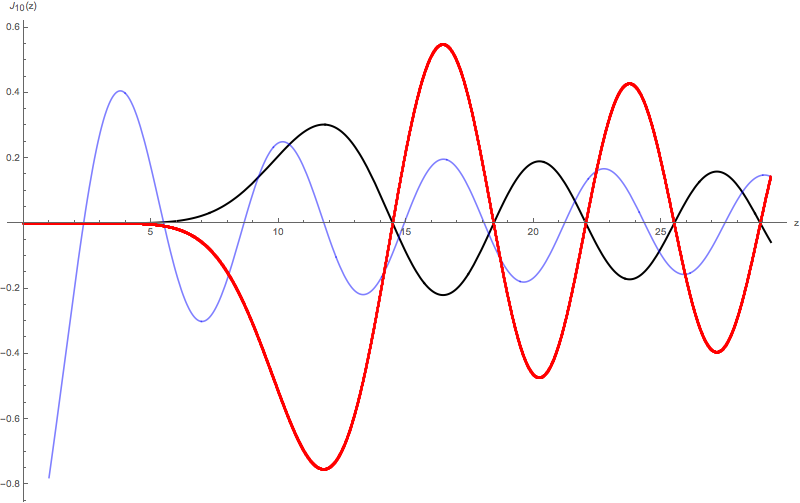
\includegraphics[width=.9\linewidth]{BesselBadBoundary.png}
  		\caption{\label{fig:BesselBadBoundary} Notice how the asymtotic form and the one calculated by our differential equation solver match up at the maximum value for $z$, but do not match up with the true solution.  This has far reaching consequences.  Whatever multiplicative factor the endpoint is off by seems to carry through for every other point.  In this case the multiplicative factor (asymtotic / true) is almost exactly $-2.5$.  Notice how this inverts the solution and makes it $250\%$ larger.}
	\end{subfigure}%
	\begin{subfigure}{.5\textwidth}
  		\centering
  		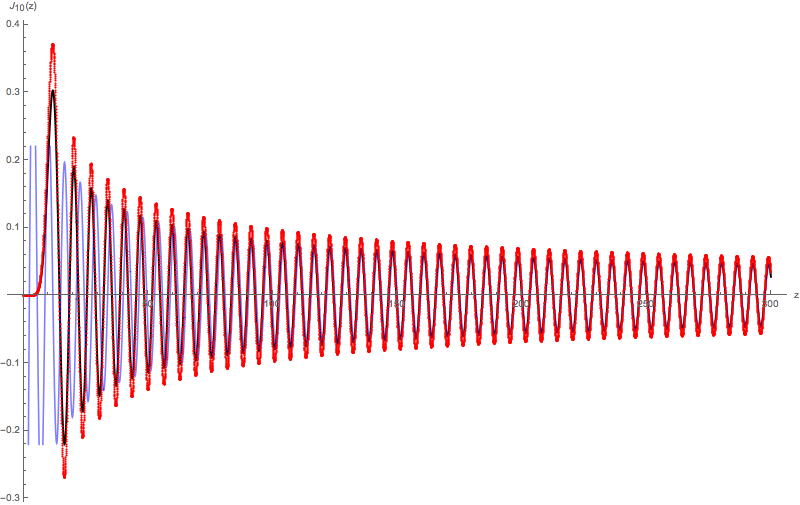
\includegraphics[width=.9\linewidth]{BesselGoodBoundary.png}
  		\caption{\label{fig:BesselGoodBoundary} For much larger values of $z$ the asymtotic form is a better approximation to the true value.  In this case the multiplicative factor (asymtotic / true evaluated at $z=300$) is roughtly $1.2$ which results in the soultion being roughly $20\%$ larger than it should be.}
	\end{subfigure}
	\caption{The blue curve is the asymtotic form of the bessel functions as given in equation \ref{eqn:asymtoticBessel}, the black curve is $J_{10} (x)$ as given by Mathematica, and the red curve is the one calculated by our differential equation solver.  Note, both of these solutions were calculated using 10,000 points.  Even though the solution in figure \ref{fig:BesselBadBoundary} has 10 times the point density, it is limited in accuracy by the endpoint!}
\end{figure*}

\subsubsection{Calculating Bessel Functions: Results}
The ultimate benchmark for sucess in calculating Bessel Functions in this manner (using the Thomas Algorithm to solve Bessel's Differential Equation) is to compare it to the stardard way of calculating the value at each point using the Riemann Sum (as defined in equation \ref{eqn:numericalIntegralBessel} section \ref{sec:boundaryConditions}).  So how much faster is it?  This depends on the values of $n$ and $z$ because we use a dynamic number of integration points as given by eq. \ref{eqn:dynamicIntegrationPoints}. Table \ref{table:besselSpeed} gives the speed increse for various parameters.

\begin{table*}[t]
	\centering
	\begin{tabular}{l || c | c | c }
		                  & Point by Point & Thomas Algo. Solving &  Speed	\\
		Parameters        & Using Integral &  Bessel's Equation   & Increse	\\
		\hline
		\hline
		n = 3             &   0.051786 s   &      0.00013800 s    &   375		\\
		N = 500           &                &                      &			\\
		$z_{max} = 20.0$  &                &                      &			\\
		\hline
		n = 14            &     113.33 s   &       0.003937 s     & 28,785	\\
		N = 50,000        &                &                      &           \\
		$z_{max} = 100.0$ &                &                      &           \\
	\end{tabular}
	\caption{\label{table:besselSpeed} $N$ is the number of points returned, $n$ is the order of the bessel function, and the points calculated were for $z \in [0,z_{max}]$ }
\end{table*}

Table \ref{fig:selectBesselFunctions} gives three examples of Bessel Functions that were calculated using the Thomas Algorithm to solve Bessel's Equation.

\begin{figure*}[t]
	\centering
	\begin{subfigure}{.5\textwidth}
  		\centering
  		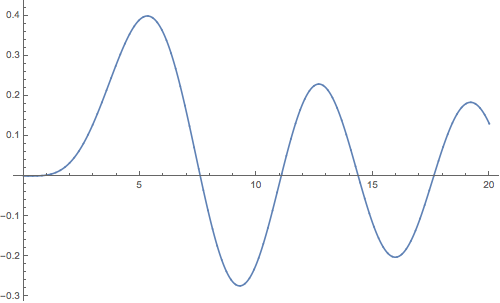
\includegraphics[width=.9\linewidth]{BesselJ4.png}
  		\caption{n=4, numPts=10,000, xMax=20, comptime=0.00082}
	\end{subfigure}%
	\begin{subfigure}{.5\textwidth}
  		\centering
  		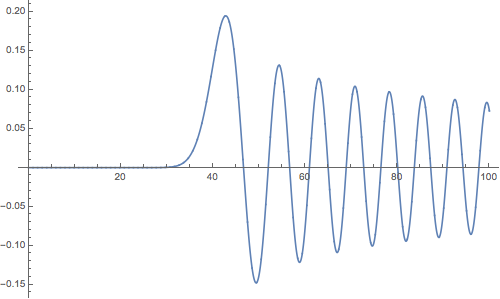
\includegraphics[width=.9\linewidth]{BesselJ40.png}
  		\caption{n=40, numPts=10,000, xMax=100, comptime=0.00092}
	\end{subfigure}
	\begin{subfigure}{.5\textwidth}
  		\centering
  		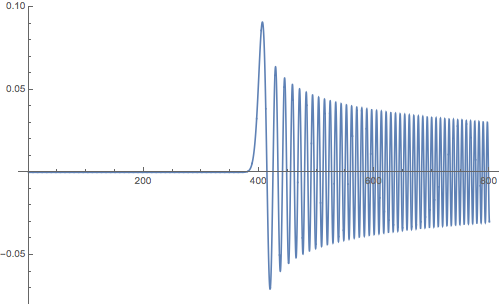
\includegraphics[width=.9\linewidth]{BesselJ400.png}
  		\caption{n=400, numPts=10,000, xMax=800, comptime=0.00200;  About half the computation time went to calculating the endpoint!}
	\end{subfigure}
	\caption{\label{fig:selectBesselFunctions}}
\end{figure*}


\begin{figure*}[t]
	\centering
	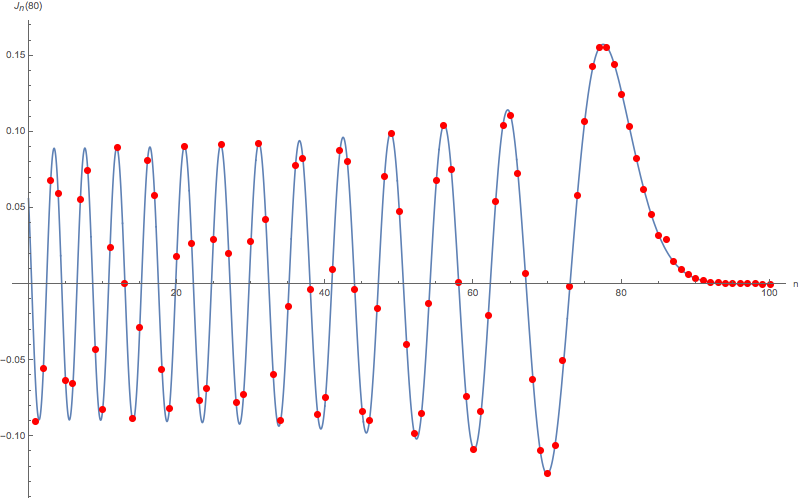
\includegraphics[width=.75\linewidth]{BesselJn80.png}
	\caption{This plot is a plot of $J_n(80)$ for values of $n\in (0,100)$.  The blue curve was generated by the BesselJ function of Mathematica.  The red dots were calculated by my code.  The two sets of data are in excelent agreement at except perhaps $n=0,85$ in which case there is a slight disagreement.  This is a small selection of the $400,000$ data points my code generated in $0.33$ seconds (on 5 year old a loptop).  It solved the Bessel differential equation for $4000$ steps in $\Gamma \in (0,100)$, then saves the output, and moved on to solve Bessel's Equation for the next value of n until all values of $\Gamma$ and n were solved for.}
\end{figure*}



\section{Conclusion}
Recap the benifits of working in the frequency domain vs the time domain.
It is the belief of this author that the methods outlined in this paper are unlikely to be useful for searching for gravitational waves.  


\appendix
\onecolumngrid
\section{The Fourier Transform of The Complex Function}
I BELIEVE I FORGOT SOME FACTORS OF 2PI HERE!!
Use the convolution theorem
Use the Jacobi-Anger expansion \ref{eqn:jacobiAnger}
Use the linearity of the Fourier Transform
Use the linearity of the Convolution
\begin{align}
\mathcal{F}_t \left[ h_0 e^{i\left( \omega_0 t + \phi_0 + \Gamma \cos( \omega_1 t + \phi_1 ) \right)} \right]
&= h_0 e^{i\phi_0} \mathcal{F}_t \left[ e^{i\omega_0 t} e^{i\Gamma \cos(\omega_1 t + \phi_1)} \right]											\\
&= h_0 e^{i\phi_0} \mathcal{F}_t \left[ e^{i\omega_0 t} \right] \star \mathcal{F}_t \left[ e^{i\Gamma \cos(\omega_1 t + \phi_1)} \right]		\\
&= h_0 e^{i\phi_0} \delta(\omega - \omega_0) 
			\star \mathcal{F}_t \left[ \sum_{n=-\infty}^{\infty} e^{in\pi/2} J_n(\Gamma) e^{in(\omega_1 t + \phi_1)} \right]							\\
&= h_0 e^{i\phi_0} \delta(\omega - \omega_0) \star \sum_{n=-\infty}^{\infty} e^{in\pi/2} e^{in\phi_1} J_n(\Gamma) F_t \left[ e^{in\omega_1 t} \right]	\\
&= h_0 e^{i\phi_0} \delta(\omega - \omega_0) \star \sum_{n=-\infty}^{\infty} e^{in(\phi_1 + \pi/2)} J_n(\Gamma) \delta(\omega - n\omega_1)			\\
&= h_0 e^{i\phi_0} \sum_{n=-\infty}^{\infty} e^{in(\phi_1 + \pi/2)} J_n(\Gamma)  \delta(\omega - \omega_0) \star \delta(\omega - n\omega_1)			\\
&= h_0 e^{i\phi_0} \sum_{n=-\infty}^{\infty} e^{in(\phi_1 + \pi/2)} J_n(\Gamma)  \delta(\omega - \omega_0 - n\omega_1)
\end{align}


\section{The Fourier Transform of The Real-Valued Function}

\begin{align}
\mathcal{F}_t \left[ \Re \left\{ h_0 e^{i\left( \omega_0 t + \phi_0 + \Gamma \cos( \omega_1 t + \phi_1 ) \right)} \right\} \right]
&= \frac{1}{2} \mathcal{F}_t \left[ h_0 e^{i\left( \omega_0 t + \phi_0 + \Gamma \cos( \omega_1 t + \phi_1 ) \right)} 
                        + h_0 e^{-i\left( \omega_0 t + \phi_0 + \Gamma \cos( \omega_1 t + \phi_1 ) \right)} \right]			\\
&= \frac{h_0}{2} \left[ 
  e^{ i\phi_0} \mathcal{F}_t \left[ e^{i\left(  \omega_0 t + \Gamma \cos( \omega_1 t + \phi_1 ) \right)} \right] 
+ e^{-i\phi_0} \mathcal{F}_t \left[ e^{i\left( -\omega_0 t - \Gamma \cos( \omega_1 t + \phi_1 ) \right)} \right] 
\right]
\end{align}

From the previous section we see that

\begin{align}
\mathcal{F}_t \left[ e^{i(\omega_0 t + \Gamma \cos(\omega_1 t + \phi_1))} \right] 
= \sum_{n=-\infty}^{\infty} e^{in(\phi_1 + \pi/2)} J_n(\Gamma)  \delta(\omega - \omega_0 - n\omega_1)
\end{align}

and by replacing $\omega_0$ with $-\omega_0$ and $\Gamma$ with $-\Gamma$, and using the fact that $J_n(-\Gamma) = (-1)^n J_n (\Gamma)$ we also have

\begin{align}
\mathcal{F}_t \left[ e^{i(-\omega_0 t - \Gamma \cos(\omega_1 t + \phi_1))} \right] 
= \sum_{n=-\infty}^{\infty} e^{in(\phi_1 - \pi/2)} J_n(\Gamma)  \delta(\omega + \omega_0 - n\omega_1)
\end{align}

so the Fourier Transform of the real part of our frequency/phase modulated signal is

\begin{align}
\begin{split}
\mathcal{F}_t \left[ \Re \left\{ h_0 e^{i\left( \omega_0 t + \phi_0 + \Gamma \cos( \omega_1 t + \phi_1 ) \right)} \right\} \right]
= \frac{1}{2} h_0 \left[ e^{ i\phi_0} \sum_{n=-\infty}^{\infty} e^{in(\phi_1 + \pi/2)} J_n(\Gamma)  \delta(\omega - \omega_0 - n\omega_1) \right.	\\
+ \left. e^{-i\phi_0} \sum_{n=-\infty}^{\infty} e^{in(\phi_1 - \pi/2)} J_n(\Gamma)  \delta(\omega + \omega_0 - n\omega_1) \right]					\\
= \frac{1}{2} h_0 \sum_{n=-\infty}^{\infty} e^{in\phi_1} J_n (\Gamma) \left[ e^{i(\phi_0 + n\pi/2)} \delta(\omega - \omega_0 - n\omega_1) \right.	\\
+ \left. e^{-i(\phi_0 + n\pi/2)} \delta(\omega + \omega_0 - n\omega_1) \right]
\end{split}
\end{align}


%\begin{align}
%\label{eqn:realFourierTransform}
%\Aboxed{\frac{1}{2} h_0 \sum_{n=-\infty}^{\infty} e^{in\phi_1} J_n (\Gamma) \left[ e^{i(\phi_0 + n\pi/2)} \delta(\omega - \omega_0 - n\omega_1)
%+ e^{-i(\phi_0 + n\pi/2)} \delta(\omega + \omega_0 - n\omega_1) \right]}
%\end{align}

\begin{align}
\label{eqn:realFourierTransform}
\hat{f}(\omega) = 
\frac{1}{2} h_0 \sum_{n=-\infty}^{\infty} e^{in\phi_1} J_n (\Gamma) \left[ e^{i(\phi_0 + n\pi/2)} \delta(\omega - \omega_0 - n\omega_1)
+ e^{-i(\phi_0 + n\pi/2)} \delta(\omega + \omega_0 - n\omega_1) \right]
\end{align}

Notice that, by taking the fourier transform of just the real part of our frequency modulated function it has added the terms in red.  (Go into more detail why that is)  The other important change is that the $X_n$ and $Y_n$ terms were added (Again, go into more detail why that is).

\section{Selected Waveforms}


\begin{figure}[H]
	\centering
	\begin{subfigure}{.5\textwidth}
  		\centering
  		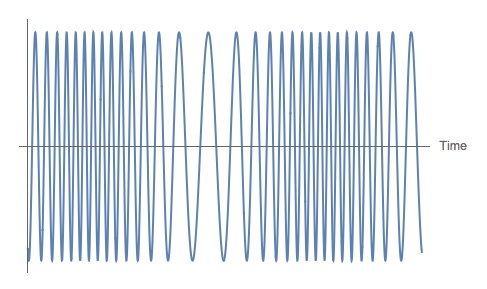
\includegraphics[width=.9\linewidth]{classicSignal.png}
  		\caption{A "nice" signal that is what comes to mind for cyclic frequency modulated signals. $\Gamma = 9.88, \omega_0 = 3.62, \omega_1 = 0.21, \phi_1 = 3.14$ \label{fig:niceSignal}}
	\end{subfigure}%
	\begin{subfigure}{.5\textwidth}
  		\centering
  		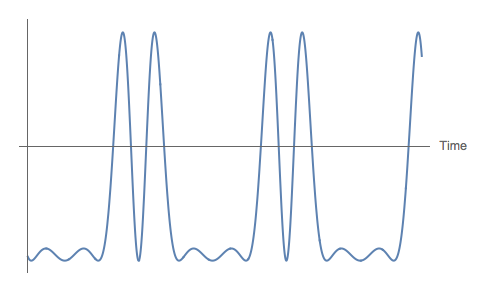
\includegraphics[width=.9\linewidth]{interestingSignal.png}
  		\caption{One example of the exotic signals cyclic frequency modulation can produce.  $\Gamma = 2.88, \omega_0 = 1.5, \omega_1 = 0.75, \phi_1 = 0$ \label{fig:interestingSignal}}
	\end{subfigure}
	\begin{subfigure}{.5\textwidth}
  		\centering
  		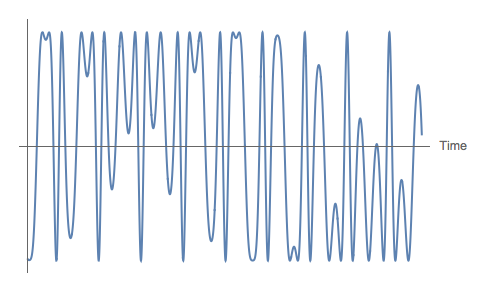
\includegraphics[width=.9\linewidth]{nastySignal.png}
  		\caption{A particularly nasty waveform that could be mistaken as noise by looking at it. $\Gamma = 3, \omega_0 = 0.42, \omega_1 = 0.46, \phi_1 = 0.1$ \label{fig:nastySignal}}
	\end{subfigure}
\end{figure}

% --------------------------- Code for the bibliography ---------------------------------------------------------------------------------
\bibliography{shgBibliographyCopy}



\end{document}